%!TEX program = xelatex
\documentclass[11pt,a4paper]{article}

% ============================================================================
% PACKAGES
% ============================================================================
\usepackage[utf8]{inputenc}
\usepackage[T1]{fontenc}
\usepackage{fontspec}
\usepackage{geometry}
\usepackage{xcolor}
\usepackage{tikz}
\usepackage{tcolorbox}
\usepackage{booktabs}
\usepackage{tabularx}
\usepackage{colortbl}
\usepackage{array}
\usepackage{multirow}
\usepackage{graphicx}
\usepackage{fancyhdr}
\usepackage{titlesec}
\usepackage{enumitem}
\usepackage{hyperref}
\usepackage{fontawesome5}
\usepackage{ragged2e}
\usepackage{setspace}
\usepackage{parskip}
\usepackage{microtype}
\usepackage{float}

% TikZ libraries
\usetikzlibrary{shapes.geometric, arrows.meta, positioning, calc, patterns, decorations.pathreplacing}

% tcolorbox libraries
\tcbuselibrary{skins,breakable}

% ============================================================================
% COLORS - Professional Business Palette
% ============================================================================
\definecolor{miloprimary}{HTML}{1E3A5F}      % Deep navy blue
\definecolor{milosecondary}{HTML}{2E86AB}    % Teal blue
\definecolor{miloaccent}{HTML}{F18F01}       % Orange accent
\definecolor{milogreen}{HTML}{2D936C}        % Success green
\definecolor{milored}{HTML}{C73E1D}          % Alert red
\definecolor{miloyellow}{HTML}{E8AA14}       % Warning yellow
\definecolor{milogray}{HTML}{6B7B8C}         % Neutral gray
\definecolor{milolight}{HTML}{F4F7FA}        % Light background
\definecolor{milodark}{HTML}{1A2530}         % Dark text

% Health score colors
\definecolor{healthgreen}{HTML}{22C55E}
\definecolor{healthlightgreen}{HTML}{84CC16}
\definecolor{healthyellow}{HTML}{EAB308}
\definecolor{healthorange}{HTML}{F97316}
\definecolor{healthred}{HTML}{EF4444}
\definecolor{healthdarkred}{HTML}{B91C1C}

% ============================================================================
% PAGE GEOMETRY
% ============================================================================
\geometry{
    a4paper,
    left=25mm,
    right=25mm,
    top=30mm,
    bottom=25mm,
    headheight=15pt
}

% ============================================================================
% FONTS
% ============================================================================
\setmainfont{Helvetica Neue}[
    UprightFont = *,
    BoldFont = * Bold,
    ItalicFont = * Italic,
    BoldItalicFont = * Bold Italic
]
\setsansfont{Helvetica Neue}

% ============================================================================
% HEADER & FOOTER
% ============================================================================
\pagestyle{fancy}
\fancyhf{}
\fancyhead[L]{\footnotesize\color{milogray}\textbf{MILO} | Business Executive Summary}
\fancyhead[R]{\footnotesize\color{milogray}Confidential}
\fancyfoot[C]{\footnotesize\color{milogray}\thepage}
\fancyfoot[R]{\footnotesize\color{milogray}DeepmAInd B.V.}
\renewcommand{\headrulewidth}{0.5pt}
\renewcommand{\headrule}{\hbox to\headwidth{\color{milosecondary}\leaders\hrule height \headrulewidth\hfill}}
\renewcommand{\footrulewidth}{0pt}

% ============================================================================
% SECTION FORMATTING
% ============================================================================
\titleformat{\section}
    {\Large\bfseries\color{miloprimary}}
    {\colorbox{miloprimary}{\textcolor{white}{\thesection}}}
    {10pt}
    {}
    [\vspace{-5pt}\textcolor{milosecondary}{\rule{\textwidth}{1pt}}]

\titleformat{\subsection}
    {\large\bfseries\color{milosecondary}}
    {\thesubsection}
    {8pt}
    {}

\titleformat{\subsubsection}
    {\normalsize\bfseries\color{milodark}}
    {\thesubsubsection}
    {6pt}
    {}

% ============================================================================
% CUSTOM BOX STYLES
% ============================================================================
\newtcolorbox{highlightbox}[1][]{
    enhanced,
    colback=milolight,
    colframe=milosecondary,
    boxrule=1pt,
    arc=4pt,
    left=10pt,
    right=10pt,
    top=10pt,
    bottom=10pt,
    fonttitle=\bfseries\color{white},
    coltitle=white,
    attach boxed title to top left={yshift=-2mm, xshift=5mm},
    boxed title style={colback=milosecondary, arc=2pt},
    #1
}

\newtcolorbox{accentbox}[1][]{
    enhanced,
    colback=miloaccent!10,
    colframe=miloaccent,
    boxrule=1.5pt,
    arc=4pt,
    left=10pt,
    right=10pt,
    top=10pt,
    bottom=10pt,
    #1
}

\newtcolorbox{keymetricbox}{
    enhanced,
    colback=miloprimary,
    colframe=miloprimary,
    boxrule=0pt,
    arc=8pt,
    left=15pt,
    right=15pt,
    top=15pt,
    bottom=15pt,
    fontupper=\color{white}
}

\newtcolorbox{riskbox}[1][]{
    enhanced,
    colback=milored!5,
    colframe=milored,
    boxrule=1pt,
    arc=4pt,
    left=10pt,
    right=10pt,
    top=10pt,
    bottom=10pt,
    #1
}

\newtcolorbox{successbox}[1][]{
    enhanced,
    colback=milogreen!5,
    colframe=milogreen,
    boxrule=1pt,
    arc=4pt,
    left=10pt,
    right=10pt,
    top=10pt,
    bottom=10pt,
    #1
}

\newtcolorbox{quotebox}{
    enhanced,
    colback=milolight,
    colframe=white,
    boxrule=0pt,
    borderline west={4pt}{0pt}{miloaccent},
    arc=0pt,
    left=15pt,
    right=10pt,
    top=10pt,
    bottom=10pt,
    fontupper=\itshape\color{milodark}
}

% ============================================================================
% HYPERREF SETUP
% ============================================================================
\hypersetup{
    colorlinks=true,
    linkcolor=milosecondary,
    urlcolor=miloaccent,
    citecolor=milogreen,
    pdftitle={MILO Business Executive Summary},
    pdfauthor={DeepmAInd B.V.},
}

% ============================================================================
% CUSTOM COMMANDS
% ============================================================================
\newcommand{\milologo}{\textcolor{miloprimary}{\textbf{MILO}}}
\newcommand{\statbox}[3]{%
    \begin{tcolorbox}[enhanced, colback=#1!15, colframe=#1, boxrule=1pt, arc=6pt, width=0.23\textwidth, halign=center, valign=center, height=2.5cm]
        {\Large\bfseries\color{#1}#2}\\[3pt]
        {\footnotesize\color{milodark}#3}
    \end{tcolorbox}%
}

\newcolumntype{L}[1]{>{\raggedright\arraybackslash}p{#1}}
\newcolumntype{C}[1]{>{\centering\arraybackslash}p{#1}}
\newcolumntype{R}[1]{>{\raggedleft\arraybackslash}p{#1}}

% ============================================================================
% DOCUMENT BEGIN
% ============================================================================
\begin{document}

% ============================================================================
% TITLE PAGE
% ============================================================================
\thispagestyle{empty}

\begin{tikzpicture}[remember picture, overlay]
    % Background gradient effect
    \fill[miloprimary] (current page.north west) rectangle ([yshift=-12cm]current page.north east);

    % Decorative elements
    \fill[milosecondary, opacity=0.3] ([xshift=5cm, yshift=-3cm]current page.north west) circle (8cm);
    \fill[miloaccent, opacity=0.2] ([xshift=-3cm, yshift=-8cm]current page.north east) circle (5cm);

    % Bottom accent bar
    \fill[miloaccent] ([yshift=2cm]current page.south west) rectangle ([yshift=2.3cm]current page.south east);
\end{tikzpicture}

\vspace*{2cm}
\begin{center}
    {\fontsize{72}{80}\selectfont\textcolor{white}{\textbf{MILO}}}\\[0.5cm]
    {\LARGE\textcolor{white!90}{Business Executive Summary v2.0}}\\[0.3cm]
    {\large\textcolor{miloaccent}{\textit{Wellness-Aware Spending Intelligence Platform}}}
\end{center}

\vspace{3cm}

\begin{center}

\begin{tikzpicture}
    % Status badges
    \node[fill=milosecondary, rounded corners=3pt, inner sep=6pt, text=white, font=\footnotesize\bfseries] at (0,0) {Status: Pre-Launch};
    \node[fill=milogreen, rounded corners=3pt, inner sep=6pt, text=white, font=\footnotesize\bfseries] at (3.5,0) {Funding: Seed Round};
    \node[fill=miloaccent, rounded corners=3pt, inner sep=6pt, text=white, font=\footnotesize\bfseries] at (7,0) {Stage: MVP Complete};
    \node[fill=milored, rounded corners=3pt, inner sep=6pt, text=white, font=\footnotesize\bfseries] at (10.5,0) {Conservative Model};
\end{tikzpicture}
\end{center}

\vfill

\begin{center}
    {\Large\textcolor{miloprimary}{\textbf{DeepmAInd B.V.}}}\\[1cm]
    \begin{tabular}{ll}
        \textcolor{milogray}{\textbf{Prepared:}} & January 28, 2026\\[3pt]
        \textcolor{milogray}{\textbf{Version:}} & 2.0 (Conservative Model)\\[3pt]
        \textcolor{milogray}{\textbf{Classification:}} & \textcolor{milored}{Confidential -- CEO Review}\\
    \end{tabular}
\end{center}

\vspace{1cm}

\newpage

% ============================================================================
% TABLE OF CONTENTS
% ============================================================================
\tableofcontents
\newpage

% ============================================================================
% SECTION 1: EXECUTIVE OVERVIEW
% ============================================================================
\section{Executive Overview}

\subsection{Company Snapshot}

\begin{center}
\begin{tabular}{>{\columncolor{milolight}}L{4cm} L{9cm}}
    \toprule
    \rowcolor{miloprimary}
    \textcolor{white}{\textbf{Attribute}} & \textcolor{white}{\textbf{Details}}\\
    \midrule
    \textbf{Company} & DeepmAInd B.V.\\
    \textbf{Product} & MILO -- AI-Powered Personal Finance App\\
    \textbf{Category} & Wellness-Aware Spending Analytics\\
    \textbf{Stage} & MVP Complete, Pre-Launch\\
    \textbf{Headquarters} & Netherlands (EU)\\
    \textbf{Funding Sought} & \$400K -- \$600K Seed\\
    \textbf{Target Launch} & Q2 2026\\
    \textbf{Projection Model} & Conservative\\
    \bottomrule
\end{tabular}
\end{center}

\subsection{Mission Statement}

\begin{quotebox}
``Empower health-conscious consumers to understand not just \textbf{how much} they spend, but \textbf{whether they're spending on healthy choices} --- while building an ethically-sourced, privacy-compliant consumer data platform.''
\end{quotebox}

\subsection{Key Highlights}

\begin{keymetricbox}
\begin{center}
{\Large\bfseries CONSERVATIVE INVESTMENT HIGHLIGHTS}\\[15pt]
\begin{tabular}{ccc}
\begin{minipage}{0.3\textwidth}
\centering
{\Huge\faIcon{bullseye}}\\[5pt]
{\large\bfseries CATEGORY CREATOR}\\[3pt]
{\small First wellness-aware spending analytics platform}
\end{minipage} &
\begin{minipage}{0.3\textwidth}
\centering
{\Huge\faIcon{dollar-sign}}\\[5pt]
{\large\bfseries \$2.4M REVENUE}\\[3pt]
{\small Year 3 projected annual revenue (conservative)}
\end{minipage} &
\begin{minipage}{0.3\textwidth}
\centering
{\Huge\faIcon{chart-line}}\\[5pt]
{\large\bfseries 58\% MARGINS}\\[3pt]
{\small Operating margins at scale (Year 3)}
\end{minipage}\\[25pt]
\begin{minipage}{0.3\textwidth}
\centering
{\Huge\faIcon{sync}}\\[5pt]
{\large\bfseries DIVERSIFIED}\\[3pt]
{\small Three distinct revenue pillars}
\end{minipage} &
\begin{minipage}{0.3\textwidth}
\centering
{\Huge\faIcon{shield-alt}}\\[5pt]
{\large\bfseries DEFENSIBLE}\\[3pt]
{\small Unique health scoring IP + privacy positioning}
\end{minipage} &
\begin{minipage}{0.3\textwidth}
\centering
{\Huge\faIcon{rocket}}\\[5pt]
{\large\bfseries 6-10x RETURN}\\[3pt]
{\small Conservative case investor return at Year 3 exit}
\end{minipage}
\end{tabular}
\end{center}
\end{keymetricbox}

\subsection{Three-Sentence Summary}

\textbf{MILO} is an AI-powered iOS application that combines receipt scanning, proprietary health scoring, and spending intelligence into a single platform --- creating an entirely new category of ``wellness-aware spending analytics.'' The company generates revenue through a three-pillar model: B2C subscriptions (35\%), B2B data monetization (52\%), and analytics reports (13\%), projecting \$2.4M in Year 3 revenue with 58\% operating margins under conservative assumptions. With \$400K-\$600K in seed funding, MILO targets 25,000 monthly active users by Year 3 and a minimum \$15M valuation at exit.

\newpage

% ============================================================================
% SECTION 2: THE OPPORTUNITY
% ============================================================================
\section{The Opportunity}

\subsection{Market Convergence}

MILO sits at the intersection of three rapidly growing markets:

\begin{center}
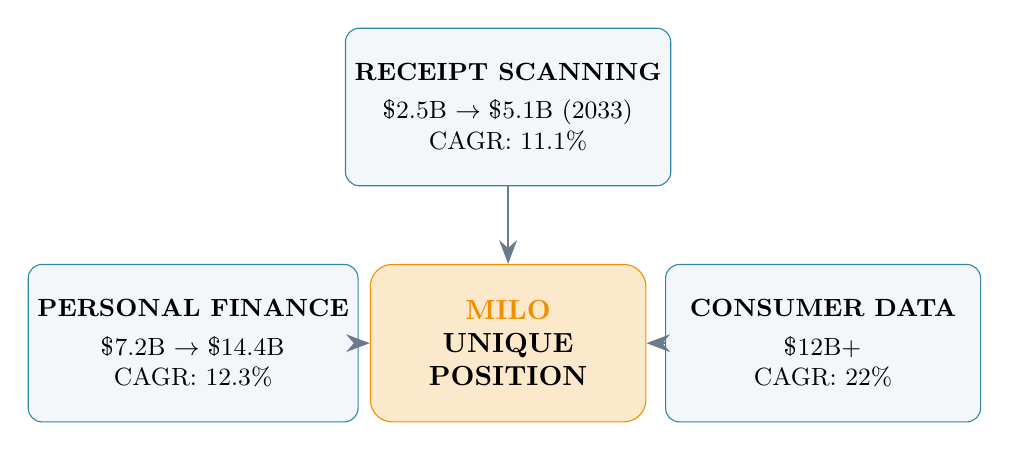
\begin{tikzpicture}[
    box/.style={draw=milosecondary, fill=milolight, rounded corners=5pt, minimum width=4cm, minimum height=2cm, align=center, font=\small},
    centerbox/.style={draw=miloaccent, fill=miloaccent!20, rounded corners=8pt, minimum width=3.5cm, minimum height=2cm, align=center, font=\bfseries},
    arrow/.style={-{Stealth[length=3mm]}, thick, milogray}
]
    % Top box
    \node[box] (receipt) at (0, 3) {\textbf{RECEIPT SCANNING}\\[3pt]\$2.5B $\rightarrow$ \$5.1B (2033)\\CAGR: 11.1\%};

    % Bottom boxes
    \node[box] (finance) at (-4, 0) {\textbf{PERSONAL FINANCE}\\[3pt]\$7.2B $\rightarrow$ \$14.4B\\CAGR: 12.3\%};
    \node[centerbox] (milo) at (0, 0) {\textcolor{miloaccent}{\textbf{MILO}}\\UNIQUE\\POSITION};
    \node[box] (data) at (4, 0) {\textbf{CONSUMER DATA}\\[3pt]\$12B+\\CAGR: 22\%};

    % Arrows
    \draw[arrow] (receipt) -- (milo);
    \draw[arrow] (finance) -- (milo);
    \draw[arrow] (data) -- (milo);
\end{tikzpicture}
\end{center}

\subsection{Total Addressable Market}

\begin{center}
\begin{tabular}{L{4.5cm} R{2.5cm} R{3cm} R{2cm}}
    \toprule
    \rowcolor{miloprimary}
    \textcolor{white}{\textbf{Market Segment}} & \textcolor{white}{\textbf{2025 Size}} & \textcolor{white}{\textbf{2030 Projection}} & \textcolor{white}{\textbf{CAGR}}\\
    \midrule
    Receipt Scanner Apps & \$2.5B & \$5.1B & 11.1\%\\
    \rowcolor{milolight}
    Personal Finance Apps & \$7.2B & \$14.4B & 12.3\%\\
    Consumer Data Analytics & \$12.0B & \$26.5B & 22.0\%\\
    \rowcolor{miloaccent!20}
    \textbf{Combined TAM} & \textbf{\$21.7B} & \textbf{\$46.0B} & \textbf{16.2\%}\\
    \bottomrule
\end{tabular}
\end{center}

\subsection{Market Catalysts}

\begin{center}
\begin{tabular}{L{3.5cm} L{5cm} R{2.5cm} C{2cm}}
    \toprule
    \rowcolor{miloprimary}
    \textcolor{white}{\textbf{Catalyst}} & \textcolor{white}{\textbf{Impact}} & \textcolor{white}{\textbf{User Base}} & \textcolor{white}{\textbf{Confidence}}\\
    \midrule
    Post-Mint Void & Users actively seeking alternatives & $\sim$3-4M & \cellcolor{miloyellow!30}Medium\\
    \rowcolor{milolight}
    Yuka Success & Proven demand for health-aware apps & 22M (US) & \cellcolor{milogreen!30}High\\
    Health Consciousness & 71\% of consumers check labels & 180M+ & \cellcolor{milogreen!30}High\\
    \rowcolor{milolight}
    AI Normalization & 73\% comfortable with AI assistants & --- & \cellcolor{milogreen!30}High\\
    GLP-1 Revolution & New health-focused consumer segment & 15M+ & \cellcolor{miloyellow!30}Medium\\
    \rowcolor{milolight}
    Subscription Fatigue & 41\% report subscription fatigue & Risk Factor & \cellcolor{milogreen!30}High\\
    \bottomrule
\end{tabular}
\end{center}

\subsection{Why Now?}

\begin{highlightbox}[title=Market Timing Assessment]
\textbf{\textcolor{milogreen}{FAVORABLE CONDITIONS:}}
\begin{itemize}[leftmargin=15pt, itemsep=2pt]
    \item[\textcolor{milogreen}{\faIcon{check}}] Health-conscious spending is mainstream (not niche)
    \item[\textcolor{milogreen}{\faIcon{check}}] AI capabilities enable 95\%+ categorization accuracy at low cost
    \item[\textcolor{milogreen}{\faIcon{check}}] Privacy regulations create premium for compliant data providers
    \item[\textcolor{milogreen}{\faIcon{check}}] Legacy competitors (Fetch, Ibotta) haven't innovated in years
    \item[\textcolor{milogreen}{\faIcon{check}}] B2B demand for consented consumer data at all-time high
\end{itemize}

\vspace{10pt}
\textbf{\textcolor{milored}{HEADWINDS TO CONSIDER:}}
\begin{itemize}[leftmargin=15pt, itemsep=2pt]
    \item[\textcolor{milored}{\faIcon{times}}] Subscription fatigue (41\% of consumers affected)
    \item[\textcolor{milored}{\faIcon{times}}] Economic uncertainty affecting discretionary spending
    \item[\textcolor{milored}{\faIcon{times}}] App Store saturation increasing CAC
    \item[\textcolor{milored}{\faIcon{times}}] Privacy regulations increasing compliance costs
\end{itemize}

\vspace{10pt}
\textbf{\textcolor{milosecondary}{NET ASSESSMENT:}} Favorable timing with manageable headwinds
\end{highlightbox}

\newpage

% ============================================================================
% SECTION 3: PRODUCT & VALUE PROPOSITION
% ============================================================================
\section{Product \& Value Proposition}

\subsection{Core Product Features}

\begin{center}
\begin{tikzpicture}
    % Header
    \node[fill=miloprimary, text=white, font=\Large\bfseries, minimum width=15cm, minimum height=1cm] at (0,0) {MILO PLATFORM};

    % Three columns
    \node[fill=milosecondary, text=white, font=\bfseries, minimum width=4.8cm, minimum height=0.8cm] at (-5,-1) {\faIcon{camera} RECEIPT SCAN};
    \node[fill=milogreen, text=white, font=\bfseries, minimum width=4.8cm, minimum height=0.8cm] at (0,-1) {\faIcon{heartbeat} HEALTH SCORES};
    \node[fill=miloaccent, text=white, font=\bfseries, minimum width=4.8cm, minimum height=0.8cm] at (5,-1) {\faIcon{robot} AI INTELLIGENCE};

    % Content boxes
    \node[fill=milolight, draw=milosecondary, rounded corners=3pt, minimum width=4.6cm, minimum height=3cm, align=left, font=\small] at (-5,-3.2) {
        \textbullet\ AI-powered OCR\\
        \textbullet\ 99\%+ accuracy\\
        \textbullet\ Instant parsing\\
        \textbullet\ Store detection\\
        \textbullet\ Item extraction
    };
    \node[fill=milolight, draw=milogreen, rounded corners=3pt, minimum width=4.6cm, minimum height=3cm, align=left, font=\small] at (0,-3.2) {
        \textbullet\ 0-5 proprietary rating\\
        \textbullet\ Food item focus\\
        \textbullet\ Nutrition-based\\
        \textbullet\ Visual display\\
        \textbullet\ Trend tracking
    };
    \node[fill=milolight, draw=miloaccent, rounded corners=3pt, minimum width=4.6cm, minimum height=3cm, align=left, font=\small] at (5,-3.2) {
        \textbullet\ Gemini 2.0 Flash\\
        \textbullet\ 95\%+ categorization\\
        \textbullet\ 16 spending categories\\
        \textbullet\ ``Milo'' chat assistant\\
        \textbullet\ Personalized insights
    };
\end{tikzpicture}
\end{center}

\subsection{Unique Value Proposition}

\begin{center}
\begin{tabular}{L{3cm} L{4.5cm} L{5cm}}
    \toprule
    \rowcolor{miloprimary}
    \textcolor{white}{\textbf{User Need}} & \textcolor{white}{\textbf{Current Solutions}} & \textcolor{white}{\textbf{MILO Advantage}}\\
    \midrule
    Track spending & Bank apps show merchants only & \textcolor{milogreen}{\textbf{Item-level granularity}}\\
    \rowcolor{milolight}
    Healthy choices & Separate nutrition apps & \textcolor{milogreen}{\textbf{Health scores on receipts}}\\
    AI insights & Generic chatbots & \textcolor{milogreen}{\textbf{Personalized spending coach}}\\
    \rowcolor{milolight}
    Data privacy & Sold without consent & \textcolor{milogreen}{\textbf{Tiered consent model}}\\
    Modern UX & Legacy interfaces & \textcolor{milogreen}{\textbf{SwiftUI native experience}}\\
    \bottomrule
\end{tabular}
\end{center}

\subsection{Health Scoring System (Proprietary IP)}

Our proprietary health scoring algorithm rates every food item on a 0-5 scale:

\begin{center}
\begin{tabular}{C{1.2cm} L{2cm} C{2cm} L{6cm}}
    \toprule
    \textbf{Score} & \textbf{Rating} & \textbf{Color} & \textbf{Description}\\
    \midrule
    \cellcolor{healthgreen!30}\textbf{5} & Excellent & \tikz\fill[healthgreen] (0,0) circle (0.3); & Whole foods, minimal processing\\
    \cellcolor{healthlightgreen!30}\textbf{4} & Good & \tikz\fill[healthlightgreen] (0,0) circle (0.3); & Healthy with minor concerns\\
    \cellcolor{healthyellow!30}\textbf{3} & Moderate & \tikz\fill[healthyellow] (0,0) circle (0.3); & Balanced, some processed elements\\
    \cellcolor{healthorange!30}\textbf{2} & Fair & \tikz\fill[healthorange] (0,0) circle (0.3); & Processed, limited nutrition\\
    \cellcolor{healthred!30}\textbf{1} & Poor & \tikz\fill[healthred] (0,0) circle (0.3); & Highly processed, low nutrition\\
    \cellcolor{healthdarkred!30}\textbf{0} & Avoid & \tikz\fill[healthdarkred] (0,0) circle (0.3); & Ultra-processed, health concerns\\
    \bottomrule
\end{tabular}
\end{center}

\subsection{Subscription Tiers (v2.0)}

\begin{center}
\begin{tabular}{L{3cm} R{2cm} C{3cm} L{4.5cm}}
    \toprule
    \rowcolor{miloprimary}
    \textcolor{white}{\textbf{Tier}} & \textcolor{white}{\textbf{Price}} & \textcolor{white}{\textbf{Receipt Limit}} & \textcolor{white}{\textbf{Key Features}}\\
    \midrule
    \faIcon{gift} \textbf{Free Trial} & \$0 (14 days) & 10 total & Try before buy\\
    \rowcolor{miloyellow!15}
    \faIcon{medal} \textbf{Gold} & \$5.99/mo & 25/month & Full analytics, 6mo history\\
    \rowcolor{milosecondary!15}
    \faIcon{gem} \textbf{Platinum} & \$12.99/mo & 50/month & Power features, 24mo history, API\\
    \bottomrule
\end{tabular}
\end{center}

\subsection{Technology Stack}

\begin{center}
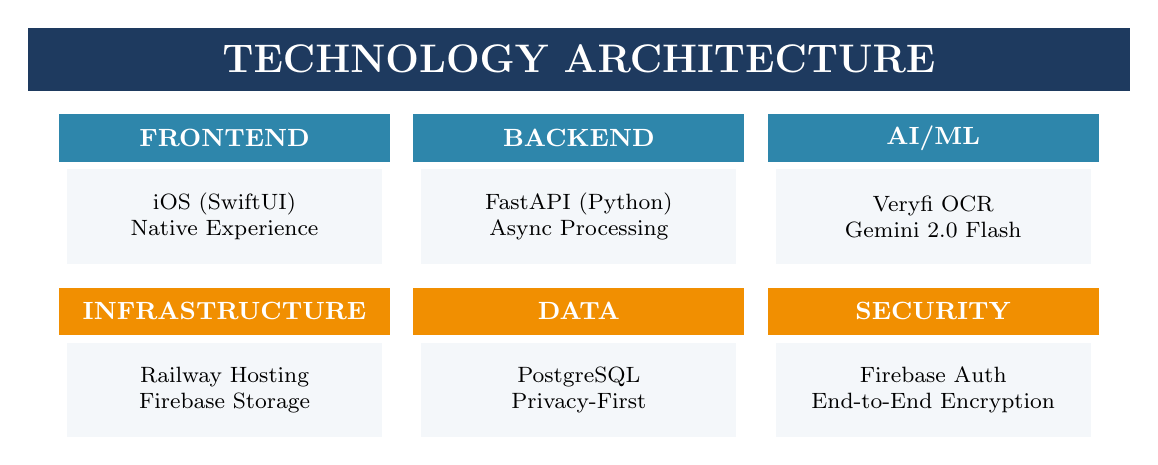
\begin{tikzpicture}
    \node[fill=miloprimary, text=white, font=\Large\bfseries, minimum width=14cm, minimum height=0.8cm] at (0,0) {TECHNOLOGY ARCHITECTURE};

    % Row 1
    \node[fill=milosecondary, text=white, font=\small\bfseries, minimum width=4.2cm, minimum height=0.6cm] at (-4.5,-1) {FRONTEND};
    \node[fill=milosecondary, text=white, font=\small\bfseries, minimum width=4.2cm, minimum height=0.6cm] at (0,-1) {BACKEND};
    \node[fill=milosecondary, text=white, font=\small\bfseries, minimum width=4.2cm, minimum height=0.6cm] at (4.5,-1) {AI/ML};

    \node[fill=milolight, font=\footnotesize, minimum width=4cm, minimum height=1.2cm, align=center] at (-4.5,-2) {iOS (SwiftUI)\\Native Experience};
    \node[fill=milolight, font=\footnotesize, minimum width=4cm, minimum height=1.2cm, align=center] at (0,-2) {FastAPI (Python)\\Async Processing};
    \node[fill=milolight, font=\footnotesize, minimum width=4cm, minimum height=1.2cm, align=center] at (4.5,-2) {Veryfi OCR\\Gemini 2.0 Flash};

    % Row 2
    \node[fill=miloaccent, text=white, font=\small\bfseries, minimum width=4.2cm, minimum height=0.6cm] at (-4.5,-3.2) {INFRASTRUCTURE};
    \node[fill=miloaccent, text=white, font=\small\bfseries, minimum width=4.2cm, minimum height=0.6cm] at (0,-3.2) {DATA};
    \node[fill=miloaccent, text=white, font=\small\bfseries, minimum width=4.2cm, minimum height=0.6cm] at (4.5,-3.2) {SECURITY};

    \node[fill=milolight, font=\footnotesize, minimum width=4cm, minimum height=1.2cm, align=center] at (-4.5,-4.2) {Railway Hosting\\Firebase Storage};
    \node[fill=milolight, font=\footnotesize, minimum width=4cm, minimum height=1.2cm, align=center] at (0,-4.2) {PostgreSQL\\Privacy-First};
    \node[fill=milolight, font=\footnotesize, minimum width=4cm, minimum height=1.2cm, align=center] at (4.5,-4.2) {Firebase Auth\\End-to-End Encryption};
\end{tikzpicture}
\end{center}

\newpage

% ============================================================================
% SECTION 4: BUSINESS MODEL
% ============================================================================
\section{Business Model}

\subsection{Three-Pillar Revenue Architecture}

\begin{center}
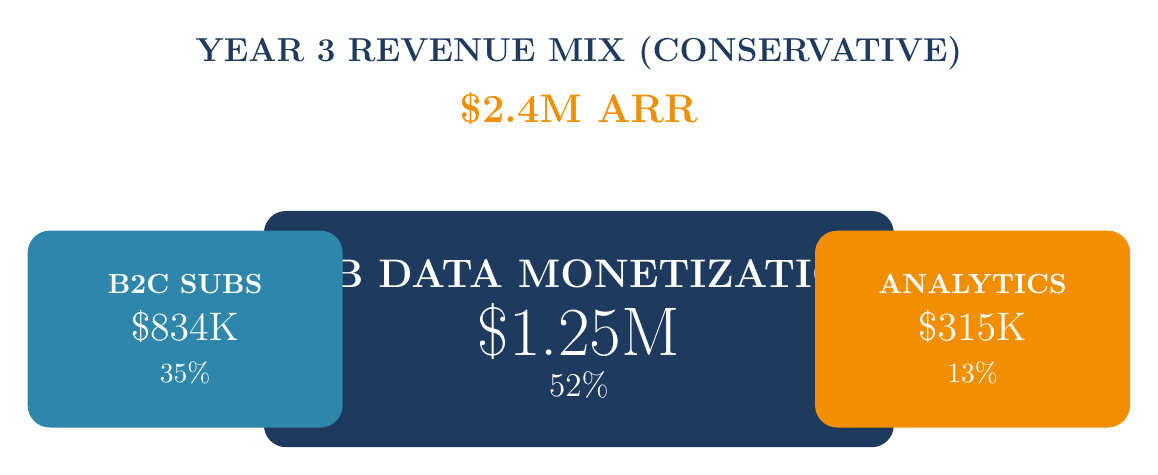
\begin{tikzpicture}
    % Title
    \node[font=\large\bfseries, color=miloprimary] at (0, 4) {YEAR 3 REVENUE MIX (CONSERVATIVE)};
    \node[font=\Large\bfseries, color=miloaccent] at (0, 3.3) {\$2.4M ARR};

    % B2B - Large center box
    \node[fill=miloprimary, text=white, minimum width=8cm, minimum height=3cm, rounded corners=8pt, align=center] (b2b) at (0, 0.5) {
        \Large\bfseries B2B DATA MONETIZATION\\[5pt]
        \Huge\$1.25M\\[3pt]
        \large 52\%
    };

    % B2C - Left box
    \node[fill=milosecondary, text=white, minimum width=4cm, minimum height=2.5cm, rounded corners=8pt, align=center] (b2c) at (-5, 0.5) {
        \bfseries B2C SUBS\\[5pt]
        \Large\$834K\\[3pt]
        35\%
    };

    % Analytics - Right box
    \node[fill=miloaccent, text=white, minimum width=4cm, minimum height=2.5cm, rounded corners=8pt, align=center] (analytics) at (5, 0.5) {
        \bfseries ANALYTICS\\[5pt]
        \Large\$315K\\[3pt]
        13\%
    };
\end{tikzpicture}
\end{center}

\subsection{Pillar 1: B2C Subscriptions (35\% of Revenue)}

\subsubsection{Subscription Tiers v2.0}

\begin{center}
\begin{tabular}{L{2.5cm} R{2cm} R{2cm} C{3cm} L{3cm}}
    \toprule
    \rowcolor{miloprimary}
    \textcolor{white}{\textbf{Tier}} & \textcolor{white}{\textbf{Monthly}} & \textcolor{white}{\textbf{Annual}} & \textcolor{white}{\textbf{Receipt Limit}} & \textcolor{white}{\textbf{Target Users}}\\
    \midrule
    \faIcon{gift} Trial & FREE & --- & 10 total (14 days) & New users exploring\\
    \rowcolor{miloyellow!15}
    \faIcon{medal} Gold & \$5.99 & \$59.99 & 25/mo & Regular shoppers\\
    \rowcolor{milosecondary!15}
    \faIcon{gem} Platinum & \$12.99 & \$129.99 & 50/mo & Power users, families\\
    \bottomrule
\end{tabular}
\end{center}

\subsubsection{Conservative Subscription Economics}

\begin{center}
\begin{tabular}{L{4cm} R{3cm} R{3cm}}
    \toprule
    \rowcolor{miloprimary}
    \textcolor{white}{\textbf{Metric}} & \textcolor{white}{\textbf{Gold}} & \textcolor{white}{\textbf{Platinum}}\\
    \midrule
    Variable Cost/User & \$2.04 & \$4.08\\
    \rowcolor{milolight}
    Gross Margin & 66.0\% & 68.6\%\\
    Expected LTV (Net) & \$50.92 & \$121.48\\
    \rowcolor{milolight}
    Monthly Churn & 10\% & 8\%\\
    Payback Period & 4.5 mo & 2.6 mo\\
    \bottomrule
\end{tabular}
\end{center}

\subsection{Pillar 2: B2B Data Monetization (52\% of Revenue)}

\subsubsection{Data Products}

\begin{center}
\begin{tabular}{L{3.5cm} L{4cm} R{2.5cm} R{2cm}}
    \toprule
    \rowcolor{miloprimary}
    \textcolor{white}{\textbf{Product}} & \textcolor{white}{\textbf{Description}} & \textcolor{white}{\textbf{Pricing}} & \textcolor{white}{\textbf{Margin}}\\
    \midrule
    \textbf{DaaS} & Per-panelist data feeds & \$25-50/user/yr & 70-80\%\\
    \rowcolor{milolight}
    \textbf{Syndicated Reports} & Quarterly trend reports & \$2K-25K each & 85-90\%\\
    \textbf{Custom Research} & Bespoke analysis & \$5K-50K & 60-70\%\\
    \bottomrule
\end{tabular}
\end{center}

\subsubsection{Conservative B2B Assumptions}

\begin{center}
\begin{tabular}{L{4cm} L{3cm} L{5cm}}
    \toprule
    \rowcolor{miloprimary}
    \textcolor{white}{\textbf{Metric}} & \textcolor{white}{\textbf{Conservative}} & \textcolor{white}{\textbf{Rationale}}\\
    \midrule
    Data Consent Rate & 40\% & Below industry average (60\%)\\
    \rowcolor{milolight}
    B2B Panelist Value & \$40/user/year & Below market rate (\$50-75)\\
    Enterprise Deals Y3 & 8-10 deals & Minimum viable pipeline\\
    \rowcolor{milolight}
    Average Deal Size & \$75K & Mid-market focus\\
    \bottomrule
\end{tabular}
\end{center}

\subsection{Pillar 3: Analytics Reports (13\% of Revenue)}

\begin{center}
\begin{tabular}{L{4cm} R{3.5cm} L{4cm}}
    \toprule
    \rowcolor{miloprimary}
    \textcolor{white}{\textbf{Report Type}} & \textcolor{white}{\textbf{Price Range}} & \textcolor{white}{\textbf{Target Buyer}}\\
    \midrule
    Quarterly Trend Reports & \$1,000 - \$3,000 & Strategy teams\\
    \rowcolor{milolight}
    Category Deep Dives & \$3,000 - \$10,000 & Brand managers\\
    Custom Market Studies & \$10,000 - \$25,000 & C-suite executives\\
    \bottomrule
\end{tabular}
\end{center}

\subsection{Revenue Concentration Risk Assessment}

\begin{riskbox}
\textbf{\textcolor{milored}{RISK:}} B2B data monetization represents 52\% of Year 3 revenue

\vspace{10pt}
\textbf{\textcolor{milogreen}{MITIGATIONS:}}
\begin{itemize}[leftmargin=15pt, itemsep=2pt]
    \item[\textcolor{milogreen}{\faIcon{check}}] B2C subscriptions provide baseline revenue (35\%)
    \item[\textcolor{milogreen}{\faIcon{check}}] B2C is not dependent on user consent for data sharing
    \item[\textcolor{milogreen}{\faIcon{check}}] Analytics reports create high-margin recurring revenue (13\%)
    \item[\textcolor{milogreen}{\faIcon{check}}] If B2B fails, business still viable at $\sim$\$1.15M revenue
\end{itemize}

\vspace{10pt}
\textbf{WORST CASE SCENARIO:}\\
If B2B revenue = \$0, B2C + Analytics = \$1.15M (Year 3)\\
Business remains operational at reduced scale
\end{riskbox}

\newpage

% ============================================================================
% SECTION 5: MARKET ANALYSIS
% ============================================================================
\section{Market Analysis}

\subsection{Target Customer Segments}

\subsubsection{B2C: Primary Segments (Conservative Sizing)}

\begin{center}
\begin{tabular}{L{4cm} R{3cm} R{2.5cm} C{2cm}}
    \toprule
    \rowcolor{miloprimary}
    \textcolor{white}{\textbf{Segment}} & \textcolor{white}{\textbf{Addressable Size}} & \textcolor{white}{\textbf{Realistic Capture}} & \textcolor{white}{\textbf{Priority}}\\
    \midrule
    \textbf{Health Optimizers} & 5M (US mobile) & 0.3\% & \cellcolor{milored!30}\textbf{HIGH}\\
    \rowcolor{milolight}
    \textbf{Ex-Mint Users} & 3M (still seeking) & 0.2\% & \cellcolor{milored!30}\textbf{HIGH}\\
    \textbf{Wellness Families} & 3M (tech-savvy) & 0.1\% & \cellcolor{miloyellow!30}MEDIUM\\
    \rowcolor{milolight}
    \textbf{Financial Optimizers} & 2M (premium) & 0.1\% & \cellcolor{miloyellow!30}MEDIUM\\
    \bottomrule
\end{tabular}
\end{center}

\subsubsection{Primary Persona: ``Healthy Hannah''}

\begin{accentbox}
\begin{center}
{\Large\bfseries\textcolor{miloaccent}{TARGET PERSONA}}
\end{center}

\vspace{10pt}

\begin{tabular}{ll@{\hspace{3cm}}ll}
    \textbf{NAME:} & Hannah Chen & \textbf{AGE:} & 32\\
    \textbf{OCCUPATION:} & Marketing Manager & \textbf{INCOME:} & \$85,000\\
    \textbf{LOCATION:} & Urban/Suburban & \textbf{TECH:} & iPhone, Apple Watch\\
\end{tabular}

\vspace{15pt}

\textbf{CURRENT APPS:} Yuka, Apple Health, MyFitnessPal

\textbf{PAIN POINTS:} Can't connect health choices to spending patterns

\textbf{WILLINGNESS:} Pays for wellness apps, values data privacy

\vspace{10pt}

\begin{quotebox}
``I want to see if my grocery budget is actually supporting my health goals''
\end{quotebox}

\textbf{MILO FIT:} Perfect alignment --- health-conscious, budget-aware, tech-savvy, willing to pay for quality tools
\end{accentbox}

\subsection{Market Sizing (Conservative)}

\begin{center}
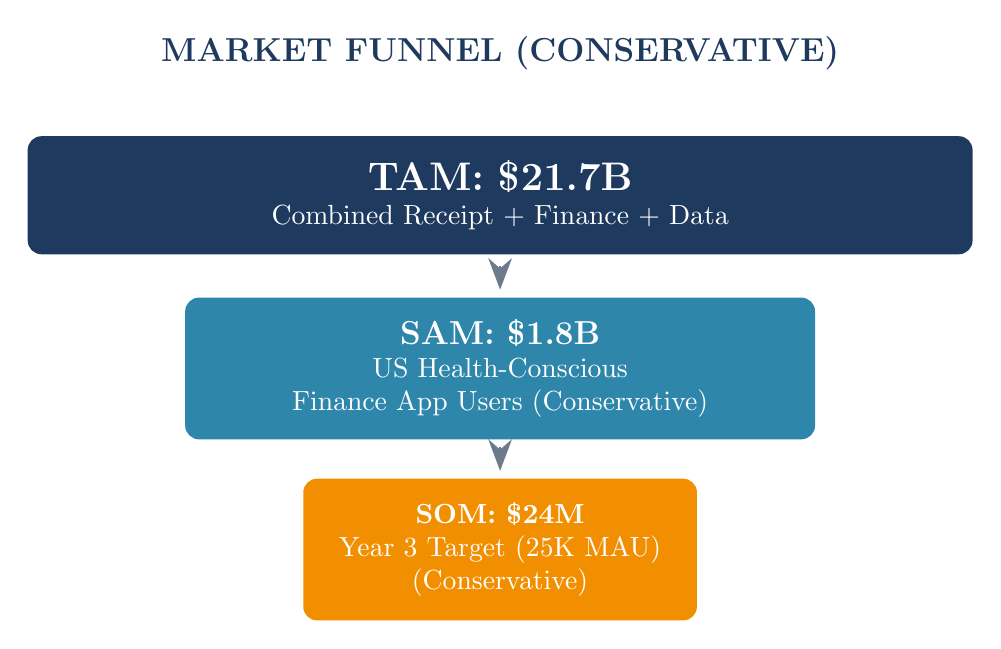
\begin{tikzpicture}
    \node[font=\large\bfseries, color=miloprimary] at (0, 5) {MARKET FUNNEL (CONSERVATIVE)};

    % TAM
    \node[fill=miloprimary, text=white, minimum width=12cm, minimum height=1.5cm, rounded corners=5pt, align=center] at (0, 3.2) {\Large\bfseries TAM: \$21.7B\\Combined Receipt + Finance + Data};

    % SAM
    \node[fill=milosecondary, text=white, minimum width=8cm, minimum height=1.8cm, rounded corners=5pt, align=center] at (0, 1) {\large\bfseries SAM: \$1.8B\\US Health-Conscious\\Finance App Users (Conservative)};

    % SOM
    \node[fill=miloaccent, text=white, minimum width=5cm, minimum height=1.8cm, rounded corners=5pt, align=center] at (0, -1.3) {\bfseries SOM: \$24M\\Year 3 Target (25K MAU)\\(Conservative)};

    % Arrows
    \draw[-{Stealth[length=4mm]}, thick, milogray] (0, 2.3) -- (0, 2);
    \draw[-{Stealth[length=4mm]}, thick, milogray] (0, 0) -- (0, -0.3);
\end{tikzpicture}
\end{center}

\newpage

% ============================================================================
% SECTION 6: FINANCIAL PROJECTIONS
% ============================================================================
\section{Financial Projections}

\subsection{3-Year Revenue Forecast (Conservative)}

\begin{center}
\begin{tabular}{L{4cm} R{2.5cm} R{2.5cm} R{2.5cm}}
    \toprule
    \rowcolor{miloprimary}
    \textcolor{white}{\textbf{Metric}} & \textcolor{white}{\textbf{Year 1}} & \textcolor{white}{\textbf{Year 2}} & \textcolor{white}{\textbf{Year 3}}\\
    \midrule
    Trial Signups & 12,500 & 35,000 & 60,000\\
    \rowcolor{milolight}
    Conversion Rate & 15\% & 17\% & 18\%\\
    Ending Paid Users & 1,688 & 5,355 & 9,720\\
    \rowcolor{milolight}
    B2C Revenue & \$128K & \$460K & \$835K\\
    B2B Revenue & \$80K & \$500K & \$1,250K\\
    \rowcolor{milolight}
    Analytics Revenue & \$20K & \$140K & \$315K\\
    \rowcolor{miloaccent!20}
    \textbf{Total Revenue} & \textbf{\$228K} & \textbf{\$1.1M} & \textbf{\$2.4M}\\
    \rowcolor{milolight}
    Operating Profit & (\$72K) & \$418K & \$1.39M\\
    \rowcolor{milogreen!20}
    \textbf{Operating Margin} & \textcolor{milored}{-31.6\%} & \textcolor{milogreen}{38.0\%} & \textcolor{milogreen}{\textbf{58.0\%}}\\
    \bottomrule
\end{tabular}
\end{center}

\subsection{Revenue Composition at Scale (Year 3)}

\begin{center}
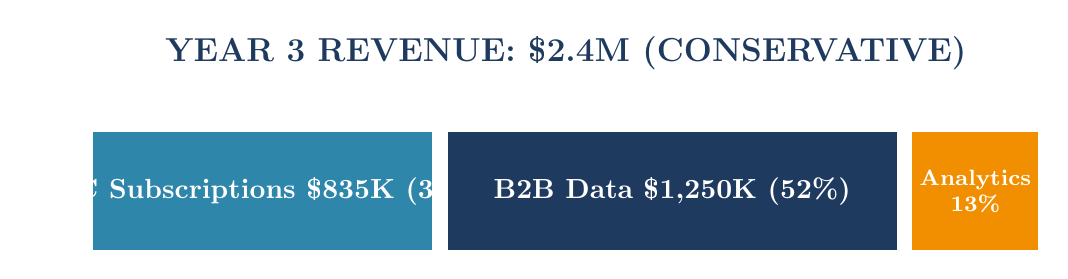
\begin{tikzpicture}
    \node[font=\large\bfseries, color=miloprimary] at (0, 2.5) {YEAR 3 REVENUE: \$2.4M (CONSERVATIVE)};

    % Stacked bars
    \fill[milosecondary] (-6, 0) rectangle (-1.7, 1.5);
    \node[text=white, font=\bfseries] at (-3.85, 0.75) {B2C Subscriptions \$835K (35\%)};

    \fill[miloprimary] (-1.5, 0) rectangle (4.2, 1.5);
    \node[text=white, font=\bfseries] at (1.35, 0.75) {B2B Data \$1,250K (52\%)};

    \fill[miloaccent] (4.4, 0) rectangle (6, 1.5);
    \node[text=white, font=\bfseries\footnotesize, align=center] at (5.2, 0.75) {Analytics\\13\%};
\end{tikzpicture}
\end{center}

\subsection{Unit Economics (Conservative)}

\begin{center}
\begin{tabular}{L{4cm} R{2.5cm} R{2.5cm} R{2.5cm}}
    \toprule
    \rowcolor{miloprimary}
    \textcolor{white}{\textbf{Metric}} & \textcolor{white}{\textbf{Gold Tier}} & \textcolor{white}{\textbf{Platinum Tier}} & \textcolor{white}{\textbf{B2B Panel}}\\
    \midrule
    Customer LTV (Net) & \$50.92 & \$121.48 & \$80.00\\
    \rowcolor{milolight}
    Customer CAC & \$17.00 & \$17.00 & \$30.00\\
    \rowcolor{milogreen!20}
    \textbf{LTV:CAC Ratio} & \textbf{3.0:1} & \textbf{7.1:1} & \textbf{2.7:1}\\
    \rowcolor{milolight}
    Payback Period & 4.5 mo & 2.6 mo & 6-8 mo\\
    \bottomrule
\end{tabular}
\end{center}

\begin{successbox}
\textbf{Assessment:} Unit economics meet minimum viability threshold (3:1) for Gold tier and significantly exceed for Platinum. B2B panel LTV:CAC is acceptable given higher margin per user.
\end{successbox}

\subsection{Profitability Milestones (Conservative)}

\begin{center}
\begin{tabular}{C{1cm} L{5cm} C{2.5cm} L{3cm}}
    \toprule
    & \textbf{Milestone} & \textbf{Timeline} & \textbf{Revenue Run-Rate}\\
    \midrule
    \cellcolor{milored!30}\textcolor{milored}{\Large\faIcon{circle}} & Break-Even (Monthly) & Month 10 & \$50K MRR\\
    \cellcolor{miloyellow!30}\textcolor{miloyellow}{\Large\faIcon{circle}} & Cash Flow Positive & Month 14 & \$80K MRR\\
    \cellcolor{milogreen!30}\textcolor{milogreen}{\Large\faIcon{circle}} & Sustained Profitability & Month 24 & \$150K MRR\\
    \bottomrule
\end{tabular}
\end{center}

\subsection{Valuation Scenarios (Year 3)}

\begin{center}
\begin{tabular}{L{3cm} C{3cm} C{3cm} C{2.5cm}}
    \toprule
    \rowcolor{miloprimary}
    \textcolor{white}{\textbf{Scenario}} & \textcolor{white}{\textbf{Revenue Multiple}} & \textcolor{white}{\textbf{Year 3 Valuation}} & \textcolor{white}{\textbf{Seed Return}}\\
    \midrule
    \textbf{Conservative} & 5x & \$12M & 3-4x\\
    \rowcolor{miloaccent!20}
    \textbf{Base Case} & 6x & \$14.4M & \textbf{6-8x}\\
    Moderate & 8x & \$19.2M & 10-12x\\
    \rowcolor{milolight}
    Optimistic & 10x & \$24M & 12-15x\\
    \bottomrule
\end{tabular}
\end{center}

\subsection{Sensitivity Analysis}

\begin{center}
\begin{tabular}{L{4cm} R{2cm} R{2cm} R{2cm} C{2cm}}
    \toprule
    \rowcolor{miloprimary}
    \textcolor{white}{\textbf{Variable}} & \textcolor{white}{\textbf{-20\%}} & \textcolor{white}{\textbf{Base}} & \textcolor{white}{\textbf{+20\%}} & \textcolor{white}{\textbf{Risk}}\\
    \midrule
    Trial Conversion & \$1.92M & \$2.4M & \$2.88M & \cellcolor{milored!30}\textbf{HIGH}\\
    \rowcolor{milolight}
    Data Consent Rate & \$2.15M & \$2.4M & \$2.65M & \cellcolor{milored!30}\textbf{HIGH}\\
    Monthly Churn & \$2.64M & \$2.4M & \$2.16M & \cellcolor{miloyellow!30}MEDIUM\\
    \rowcolor{milolight}
    B2B Deal Size & \$2.25M & \$2.4M & \$2.55M & \cellcolor{miloyellow!30}MEDIUM\\
    Veryfi Costs & \$2.44M & \$2.4M & \$2.36M & \cellcolor{milogreen!30}LOW\\
    \bottomrule
\end{tabular}
\end{center}

\newpage

% ============================================================================
% SECTION 7: GO-TO-MARKET STRATEGY
% ============================================================================
\section{Go-to-Market Strategy}

\subsection{Launch Timeline}

\begin{center}
\begin{tikzpicture}[
    phase/.style={draw=milosecondary, fill=milolight, rounded corners=8pt, minimum width=3.2cm, minimum height=4cm, align=center},
    arrow/.style={-{Stealth[length=4mm]}, thick, miloaccent}
]
    \node[font=\large\bfseries, color=miloprimary] at (0, 3.5) {GO-TO-MARKET PHASES (CONSERVATIVE)};

    % Phase boxes
    \node[phase] (p1) at (-5.5, 0) {
        \textbf{\textcolor{milosecondary}{PRE-LAUNCH}}\\
        {\footnotesize(M-3 to M0)}\\[8pt]
        {\small\faIcon{check} ASO Setup}\\
        {\small\faIcon{check} Beta Program}\\
        {\small\faIcon{check} Waitlist (500)}\\
        {\small\faIcon{check} Content}\\[8pt]
        {\footnotesize\textcolor{milogray}{Target: 300 Beta}}
    };

    \node[phase] (p2) at (-1.8, 0) {
        \textbf{\textcolor{milosecondary}{LAUNCH}}\\
        {\footnotesize(M1-M6)}\\[8pt]
        {\small\faIcon{check} Soft Launch}\\
        {\small\faIcon{check} PR Push}\\
        {\small\faIcon{check} Paid Ads}\\
        {\small\faIcon{check} Influencers}\\[8pt]
        {\footnotesize\textcolor{milogray}{Target: 1.5K MAU}}
    };

    \node[phase] (p3) at (1.9, 0) {
        \textbf{\textcolor{milosecondary}{SCALE}}\\
        {\footnotesize(M7-M18)}\\[8pt]
        {\small\faIcon{check} CAC < \$20}\\
        {\small\faIcon{check} 2 B2B Pilots}\\
        {\small\faIcon{check} 25\% Organic}\\
        {\small\faIcon{check} 5K MAU}\\[8pt]
        {\footnotesize\textcolor{milogray}{Target: 7K MAU}}
    };

    \node[phase] (p4) at (5.6, 0) {
        \textbf{\textcolor{milosecondary}{EXPAND}}\\
        {\footnotesize(M19-36)}\\[8pt]
        {\small\faIcon{check} Android}\\
        {\small\faIcon{check} UK Market}\\
        {\small\faIcon{check} Enterprise}\\
        {\small\faIcon{check} 15K MAU}\\[8pt]
        {\footnotesize\textcolor{milogray}{Target: 25K MAU}}
    };

    % Arrows
    \draw[arrow] (p1) -- (p2);
    \draw[arrow] (p2) -- (p3);
    \draw[arrow] (p3) -- (p4);
\end{tikzpicture}
\end{center}

\subsection{Marketing Budget Allocation (Year 1: \$75K)}

\begin{center}
\begin{tabular}{C{1cm} L{4cm} C{2cm} R{2cm} L{4cm}}
    \toprule
    & \textbf{Channel} & \textbf{Allocation} & \textbf{Budget} & \textbf{Focus}\\
    \midrule
    \faIcon{mobile-alt} & Paid Acquisition & 35\% & \$26,250 & App installs, retargeting\\
    \rowcolor{milolight}
    \faIcon{bullseye} & Influencer Marketing & 20\% & \$15,000 & Micro partnerships\\
    \faIcon{pen} & Content \& SEO & 20\% & \$15,000 & Organic growth engine\\
    \rowcolor{milolight}
    \faIcon{building} & B2B Marketing & 15\% & \$11,250 & ABM, thought leadership\\
    \faIcon{palette} & Brand \& Creative & 10\% & \$7,500 & Assets, video production\\
    \bottomrule
\end{tabular}
\end{center}

\subsection{Key Performance Targets (Conservative)}

\begin{center}
\begin{tabular}{L{3.5cm} R{2cm} R{2cm} R{2cm} R{2cm}}
    \toprule
    \rowcolor{miloprimary}
    \textcolor{white}{\textbf{Metric}} & \textcolor{white}{\textbf{M6}} & \textcolor{white}{\textbf{M12}} & \textcolor{white}{\textbf{M24}} & \textcolor{white}{\textbf{M36}}\\
    \midrule
    MAU & 1,500 & 3,500 & 9,000 & 25,000\\
    \rowcolor{milolight}
    Paid Users & 225 & 525 & 1,350 & 3,750\\
    CAC & \$30 & \$22 & \$18 & \$15\\
    \rowcolor{milolight}
    Organic \% & 15\% & 25\% & 35\% & 45\%\\
    D7 Retention & 35\%+ & 38\%+ & 40\%+ & 42\%+\\
    \rowcolor{milolight}
    D30 Retention & 20\%+ & 22\%+ & 25\%+ & 28\%+\\
    \bottomrule
\end{tabular}
\end{center}

\newpage

% ============================================================================
% SECTION 8: COMPETITIVE POSITIONING
% ============================================================================
\section{Competitive Positioning}

\subsection{Competitive Landscape}

\begin{center}
\begin{tabular}{L{3cm} R{1.8cm} R{1.8cm} L{3cm} C{1.5cm} C{1.5cm}}
    \toprule
    \rowcolor{miloprimary}
    \textcolor{white}{\textbf{Competitor}} & \textcolor{white}{\textbf{Users}} & \textcolor{white}{\textbf{Valuation}} & \textcolor{white}{\textbf{Focus}} & \textcolor{white}{\textbf{Health}} & \textcolor{white}{\textbf{Threat}}\\
    \midrule
    Fetch Rewards & 12.5M & \$2.5B & Rewards/Points & \textcolor{milored}{\faIcon{times}} & \cellcolor{miloyellow!30}Med\\
    \rowcolor{milolight}
    Ibotta & 14.7M & \$800M+ & Cashback & \textcolor{milored}{\faIcon{times}} & \cellcolor{miloyellow!30}Med\\
    Receipt Hog & 10M+ & Private & Gamified & \textcolor{milored}{\faIcon{times}} & \cellcolor{milogreen!30}Low\\
    \rowcolor{milolight}
    Copilot & N/A & N/A & AI Budgeting & \textcolor{milored}{\faIcon{times}} & \cellcolor{miloyellow!30}Med\\
    Monarch Money & Growing & N/A & Household & \textcolor{milored}{\faIcon{times}} & \cellcolor{miloyellow!30}Med\\
    \rowcolor{miloaccent!20}
    \textbf{MILO} & Pre-launch & --- & Wellness+Finance & \textcolor{milogreen}{\faIcon{check}} & ---\\
    \bottomrule
\end{tabular}
\end{center}

\subsection{Competitive Matrix}

\begin{center}
\begin{tikzpicture}
    \node[font=\large\bfseries, color=miloprimary] at (0, 2) {FEATURE COMPARISON};

    % Header row
    \node[fill=miloprimary, text=white, minimum width=2.8cm, minimum height=0.7cm, font=\small\bfseries] at (-4.5, 1) {};
    \node[fill=miloprimary, text=white, minimum width=2.8cm, minimum height=0.7cm, font=\footnotesize\bfseries] at (-1.5, 1) {Item-Level};
    \node[fill=miloprimary, text=white, minimum width=2.8cm, minimum height=0.7cm, font=\footnotesize\bfseries] at (1.5, 1) {Health Scoring};
    \node[fill=miloprimary, text=white, minimum width=2.8cm, minimum height=0.7cm, font=\footnotesize\bfseries] at (4.5, 1) {AI Chat};
    \node[fill=miloprimary, text=white, minimum width=2.8cm, minimum height=0.7cm, font=\footnotesize\bfseries] at (7.5, 1) {Privacy};

    % MILO row
    \node[fill=miloaccent!20, minimum width=2.8cm, minimum height=0.6cm, font=\small\bfseries] at (-4.5, 0.3) {MILO};
    \node[fill=miloaccent!20, minimum width=2.8cm, minimum height=0.6cm] at (-1.5, 0.3) {\textcolor{milogreen}{\Large\faIcon{check-circle}}};
    \node[fill=miloaccent!20, minimum width=2.8cm, minimum height=0.6cm] at (1.5, 0.3) {\textcolor{milogreen}{\Large\faIcon{check-circle}}};
    \node[fill=miloaccent!20, minimum width=2.8cm, minimum height=0.6cm] at (4.5, 0.3) {\textcolor{milogreen}{\Large\faIcon{check-circle}}};
    \node[fill=miloaccent!20, minimum width=2.8cm, minimum height=0.6cm] at (7.5, 0.3) {\textcolor{milogreen}{\Large\faIcon{check-circle}}};

    % Other rows
    \foreach \name/\y in {Fetch Rewards/-0.4, Ibotta/-1.1, Copilot/-1.8, Monarch/-2.5} {
        \node[fill=milolight, minimum width=2.8cm, minimum height=0.6cm, font=\small] at (-4.5, \y) {\name};
        \node[fill=milolight, minimum width=2.8cm, minimum height=0.6cm] at (-1.5, \y) {\textcolor{milored}{\Large\faIcon{times-circle}}};
        \node[fill=milolight, minimum width=2.8cm, minimum height=0.6cm] at (1.5, \y) {\textcolor{milored}{\Large\faIcon{times-circle}}};
    }
    \node[fill=milolight, minimum width=2.8cm, minimum height=0.6cm] at (4.5, -0.4) {\textcolor{milored}{\Large\faIcon{times-circle}}};
    \node[fill=milolight, minimum width=2.8cm, minimum height=0.6cm] at (7.5, -0.4) {\textcolor{milored}{\Large\faIcon{times-circle}}};
    \node[fill=milolight, minimum width=2.8cm, minimum height=0.6cm] at (4.5, -1.1) {\textcolor{milored}{\Large\faIcon{times-circle}}};
    \node[fill=milolight, minimum width=2.8cm, minimum height=0.6cm] at (7.5, -1.1) {\textcolor{milored}{\Large\faIcon{times-circle}}};
    \node[fill=milolight, minimum width=2.8cm, minimum height=0.6cm] at (4.5, -1.8) {\textcolor{milogreen}{\Large\faIcon{check-circle}}};
    \node[fill=milolight, minimum width=2.8cm, minimum height=0.6cm] at (7.5, -1.8) {\textcolor{miloyellow}{\Large\faIcon{exclamation-circle}}};
    \node[fill=milolight, minimum width=2.8cm, minimum height=0.6cm] at (4.5, -2.5) {\textcolor{milored}{\Large\faIcon{times-circle}}};
    \node[fill=milolight, minimum width=2.8cm, minimum height=0.6cm] at (7.5, -2.5) {\textcolor{miloyellow}{\Large\faIcon{exclamation-circle}}};
\end{tikzpicture}
\end{center}

\subsection{SWOT Analysis}

\begin{center}
\begin{tikzpicture}
    % Strengths
    \node[fill=milogreen!20, draw=milogreen, rounded corners=5pt, minimum width=7cm, minimum height=4cm, align=left, anchor=north west, font=\small] at (-7.2, 0) {
        \textbf{\textcolor{milogreen}{STRENGTHS}}\\[5pt]
        \faIcon{check} Unique health scoring IP\\
        \faIcon{check} Modern AI tech (cost savings)\\
        \faIcon{check} Privacy-first architecture\\
        \faIcon{check} Dual B2C + B2B revenue\\
        \faIcon{check} Item-level data granularity
    };

    % Weaknesses
    \node[fill=milored!20, draw=milored, rounded corners=5pt, minimum width=7cm, minimum height=4cm, align=left, anchor=north west, font=\small] at (0.2, 0) {
        \textbf{\textcolor{milored}{WEAKNESSES}}\\[5pt]
        \faIcon{times} No existing user base\\
        \faIcon{times} iOS-only (57\% addressable)\\
        \faIcon{times} No rewards/cashback\\
        \faIcon{times} Limited brand awareness\\
        \faIcon{times} Requires external funding\\
        \faIcon{times} Small team capacity
    };

    % Opportunities
    \node[fill=milosecondary!20, draw=milosecondary, rounded corners=5pt, minimum width=7cm, minimum height=3.5cm, align=left, anchor=north west, font=\small] at (-7.2, -4.3) {
        \textbf{\textcolor{milosecondary}{OPPORTUNITIES}}\\[5pt]
        \faIcon{arrow-up} Health-conscious trend (71\%)\\
        \faIcon{arrow-up} B2B data demand growing\\
        \faIcon{arrow-up} AI normalization (73\%)\\
        \faIcon{arrow-up} GLP-1 awareness (16\% HH)
    };

    % Threats
    \node[fill=miloyellow!20, draw=miloyellow, rounded corners=5pt, minimum width=7cm, minimum height=3.5cm, align=left, anchor=north west, font=\small] at (0.2, -4.3) {
        \textbf{\textcolor{miloyellow}{THREATS}}\\[5pt]
        \faIcon{arrow-down} Big Tech entry risk (Apple)\\
        \faIcon{arrow-down} Economic downturn impact\\
        \faIcon{arrow-down} Privacy regulation tightening\\
        \faIcon{arrow-down} Subscription fatigue (41\%)\\
        \faIcon{arrow-down} CAC inflation trend
    };
\end{tikzpicture}
\end{center}

\newpage

% ============================================================================
% SECTION 9: RISK ASSESSMENT
% ============================================================================
\section{Risk Assessment}

\subsection{Risk Summary}

\begin{center}
\begin{tabular}{L{3cm} C{2cm} C{2cm} C{2cm} C{2cm}}
    \toprule
    \rowcolor{miloprimary}
    \textcolor{white}{\textbf{Category}} & \textcolor{white}{\textbf{Critical}} & \textcolor{white}{\textbf{High}} & \textcolor{white}{\textbf{Medium}} & \textcolor{white}{\textbf{Low}}\\
    \midrule
    Market & 0 & 2 & 2 & 1\\
    \rowcolor{milolight}
    Technical & 0 & 1 & 2 & 1\\
    Financial & 1 & 1 & 1 & 0\\
    \rowcolor{milolight}
    Regulatory & 1 & 1 & 1 & 0\\
    \rowcolor{milored!20}
    \textbf{Total} & \textbf{2} & \textbf{5} & \textbf{6} & \textbf{2}\\
    \bottomrule
\end{tabular}
\end{center}

\subsection{Critical Risks}

\begin{riskbox}
\textbf{\Large\textcolor{milored}{Risk 1: GDPR Non-Compliance at Launch}}

\vspace{10pt}
\begin{tabular}{L{3cm} L{9cm}}
    \textbf{Impact} & CRITICAL (Cannot launch in EU, 52\% of revenue blocked)\\
    \textbf{Probability} & MEDIUM (If timeline slips)\\
    \textbf{Current Status} & 25/100 readiness score\\
    \textbf{Mitigation} & Dedicated \texteuro75K-115K budget, 12-week remediation plan\\
    \textbf{Residual Risk} & LOW after mitigation\\
\end{tabular}
\end{riskbox}

\vspace{10pt}

\begin{riskbox}
\textbf{\Large\textcolor{milored}{Risk 2: Insufficient Seed Funding}}

\vspace{10pt}
\begin{tabular}{L{3cm} L{9cm}}
    \textbf{Impact} & CRITICAL (Operations cease)\\
    \textbf{Probability} & MEDIUM\\
    \textbf{Mitigation} & Conservative projections, multiple investor outreach, lean ops\\
    \textbf{Residual Risk} & MEDIUM\\
\end{tabular}
\end{riskbox}

\subsection{High-Priority Risks}

\begin{center}
\begin{tabular}{L{4.5cm} C{1.5cm} C{2cm} L{4.5cm}}
    \toprule
    \rowcolor{miloprimary}
    \textcolor{white}{\textbf{Risk}} & \textcolor{white}{\textbf{Impact}} & \textcolor{white}{\textbf{Probability}} & \textcolor{white}{\textbf{Mitigation}}\\
    \midrule
    User data consent <40\% & HIGH & MEDIUM & Value exchange, gradual consent\\
    \rowcolor{milolight}
    Trial conversion <15\% & HIGH & MEDIUM & A/B testing, offer optimization\\
    Veryfi API cost increase & HIGH & LOW & Volume contracts, alternatives\\
    \rowcolor{milolight}
    Big Tech competitive entry & HIGH & LOW & Speed to market, niche focus\\
    Key personnel departure & HIGH & LOW & Equity incentives, documentation\\
    \bottomrule
\end{tabular}
\end{center}

\subsection{Overall Risk Profile}

\begin{highlightbox}[title=Risk Assessment]
\textbf{\Large MODERATE-HIGH RISK}

\vspace{10pt}
Two critical risks identified (GDPR compliance, funding). Business model viable but requires execution excellence and sufficient capital. Conservative projections provide buffer for underperformance.
\end{highlightbox}

\newpage

% ============================================================================
% SECTION 10: COMPLIANCE & LEGAL
% ============================================================================
\section{Compliance \& Legal}

\subsection{GDPR Compliance Status}

\begin{keymetricbox}
\begin{center}
{\Large\bfseries GDPR READINESS ASSESSMENT}\\[15pt]
\begin{tabular}{ll}
    \textbf{Current Status:} & \textcolor{milored}{\textbf{NON-COMPLIANT}}\\[5pt]
    \textbf{Readiness Score:} & 25/100\\[5pt]
    \textbf{Required Investment:} & \texteuro75K - 115K\\[5pt]
    \textbf{Timeline to Compliance:} & 12 weeks\\
\end{tabular}

\vspace{15pt}
\textcolor{miloyellow}{\faIcon{exclamation-triangle}} \textbf{CRITICAL: Cannot launch or monetize data without GDPR compliance}
\end{center}
\end{keymetricbox}

\subsection{Compliance Priorities}

\begin{center}
\begin{tabular}{C{1.5cm} L{5cm} C{2cm} R{2.5cm}}
    \toprule
    \textbf{Priority} & \textbf{Requirement} & \textbf{Status} & \textbf{Investment}\\
    \midrule
    \cellcolor{milored!30}\textbf{Critical} & Privacy Policy & \textcolor{milored}{\faIcon{times} Missing} & \texteuro5-10K\\
    \cellcolor{milored!30}\textbf{Critical} & Data Processing Agreements & \textcolor{milored}{\faIcon{times} Missing} & \texteuro15-25K\\
    \cellcolor{milored!30}\textbf{Critical} & Consent Management System & \textcolor{milored}{\faIcon{times} Missing} & \texteuro10-15K\\
    \cellcolor{miloyellow!30}\textbf{High} & Data Subject Rights Portal & \textcolor{milored}{\faIcon{times} Missing} & \texteuro15-20K\\
    \cellcolor{miloyellow!30}\textbf{High} & International Transfer Docs & \textcolor{milored}{\faIcon{times} Missing} & \texteuro10-15K\\
    \cellcolor{miloyellow!30}\textbf{High} & DPIA for AI Processing & \textcolor{milored}{\faIcon{times} Missing} & \texteuro10-15K\\
    \bottomrule
\end{tabular}
\end{center}

\subsection{Compliance Roadmap}

\begin{center}
\begin{tikzpicture}[
    phase/.style={draw=milosecondary, fill=milolight, rounded corners=8pt, minimum width=4.5cm, minimum height=4.5cm, align=center}
]
    \node[phase] (p1) at (-5, 0) {
        \textbf{\textcolor{milosecondary}{PHASE 1}}\\
        {\footnotesize Foundation}\\
        {\footnotesize(Weeks 1-4)}\\[10pt]
        {\small\faIcon{check} Privacy Policy}\\
        {\small\faIcon{check} Legal Basis Docs}\\
        {\small\faIcon{check} DPA Execution}\\
        {\small\faIcon{check} Transfer Mechs}\\[10pt]
        {\footnotesize\textcolor{miloaccent}{\texteuro35K-50K}}
    };

    \node[phase] (p2) at (0, 0) {
        \textbf{\textcolor{milosecondary}{PHASE 2}}\\
        {\footnotesize Rights \& Controls}\\
        {\footnotesize(Weeks 5-8)}\\[10pt]
        {\small\faIcon{check} Rights Portal}\\
        {\small\faIcon{check} Consent UI}\\
        {\small\faIcon{check} Export Function}\\
        {\small\faIcon{check} Deletion Flow}\\[10pt]
        {\footnotesize\textcolor{miloaccent}{\texteuro25K-40K}}
    };

    \node[phase] (p3) at (5, 0) {
        \textbf{\textcolor{milosecondary}{PHASE 3}}\\
        {\footnotesize Governance}\\
        {\footnotesize(Weeks 9-12)}\\[10pt]
        {\small\faIcon{check} Audit Process}\\
        {\small\faIcon{check} Training}\\
        {\small\faIcon{check} Documentation}\\
        {\small\faIcon{check} Monitoring}\\[10pt]
        {\footnotesize\textcolor{miloaccent}{\texteuro15K-25K}}
    };

    \draw[-{Stealth[length=4mm]}, thick, miloaccent] (p1) -- (p2);
    \draw[-{Stealth[length=4mm]}, thick, miloaccent] (p2) -- (p3);
\end{tikzpicture}
\end{center}

\newpage

% ============================================================================
% SECTION 11: INVESTMENT THESIS
% ============================================================================
\section{Investment Thesis}

\subsection{Investment Summary}

\begin{keymetricbox}
\begin{center}
{\Large\bfseries INVESTMENT OPPORTUNITY (CONSERVATIVE)}\\[20pt]
\begin{tabular}{ll}
    \textbf{AMOUNT SOUGHT:} & \$400,000 -- \$600,000\\[8pt]
    \textbf{ROUND:} & Seed\\[8pt]
    \textbf{USE:} & Product, Compliance, Growth, Operations\\[8pt]
    \textbf{RUNWAY:} & 18-24 months\\[8pt]
    \textbf{TARGET RETURN:} & 6-10x at Year 3 exit (conservative)\\
\end{tabular}
\end{center}
\end{keymetricbox}

\subsection{Use of Funds (\$500K Mid-Point)}

\begin{center}
\begin{tabular}{C{1cm} L{4cm} C{1.5cm} R{2cm} L{4.5cm}}
    \toprule
    & \textbf{Category} & \textbf{\%} & \textbf{Amount} & \textbf{Purpose}\\
    \midrule
    \faIcon{laptop-code} & Product Development & 30\% & \$150K & Subscriptions, B2B features, infra\\
    \rowcolor{milolight}
    \faIcon{balance-scale} & Legal \& Compliance & 20\% & \$100K & GDPR, privacy, data agreements\\
    \faIcon{bullhorn} & User Acquisition & 20\% & \$100K & Marketing, influencers, paid\\
    \rowcolor{milolight}
    \faIcon{handshake} & B2B Sales & 15\% & \$75K & Sales capability, partnerships\\
    \faIcon{building} & Operations & 15\% & \$75K & Finance, HR, admin, contingency\\
    \bottomrule
\end{tabular}
\end{center}

\begin{center}

\begin{tikzpicture}
    % Stacked bar chart
    \fill[milosecondary] (0, 0) rectangle (4.5, 0.8);
    \fill[milogreen] (4.5, 0) rectangle (7.5, 0.8);
    \fill[miloaccent] (7.5, 0) rectangle (10.5, 0.8);
    \fill[miloprimary] (10.5, 0) rectangle (12.75, 0.8);
    \fill[milogray] (12.75, 0) rectangle (15, 0.8);

    \node[text=white, font=\footnotesize\bfseries] at (2.25, 0.4) {Product 30\%};
    \node[text=white, font=\footnotesize\bfseries] at (6, 0.4) {Legal 20\%};
    \node[text=white, font=\footnotesize\bfseries] at (9, 0.4) {UA 20\%};
    \node[text=white, font=\footnotesize\bfseries] at (11.6, 0.4) {B2B 15\%};
    \node[text=white, font=\footnotesize\bfseries] at (13.9, 0.4) {Ops 15\%};
\end{tikzpicture}
\end{center}

\subsection{Investment Highlights}

\begin{center}
\begin{tabular}{C{1cm} L{4cm} L{8cm}}
    \toprule
    & \textbf{Factor} & \textbf{Details}\\
    \midrule
    \faIcon{bullseye} & \textbf{Category Creation} & First wellness-aware spending analytics platform\\
    \rowcolor{milolight}
    \faIcon{dollar-sign} & \textbf{Sustainable Economics} & 58\% operating margins, 3:1+ LTV:CAC\\
    \faIcon{sync} & \textbf{Diversified Revenue} & Three pillars reduce concentration risk\\
    \rowcolor{milolight}
    \faIcon{shield-alt} & \textbf{Moderate Moat} & Health scoring IP, privacy positioning\\
    \faIcon{chart-line} & \textbf{Achievable Milestones} & Conservative targets within reach\\
    \rowcolor{milolight}
    \faIcon{bolt} & \textbf{Capital Efficiency} & Profitable by Month 14, 18-24mo runway\\
    \bottomrule
\end{tabular}
\end{center}

\subsection{Exit Strategy}

\subsubsection{Potential Strategic Acquirers}

\begin{center}
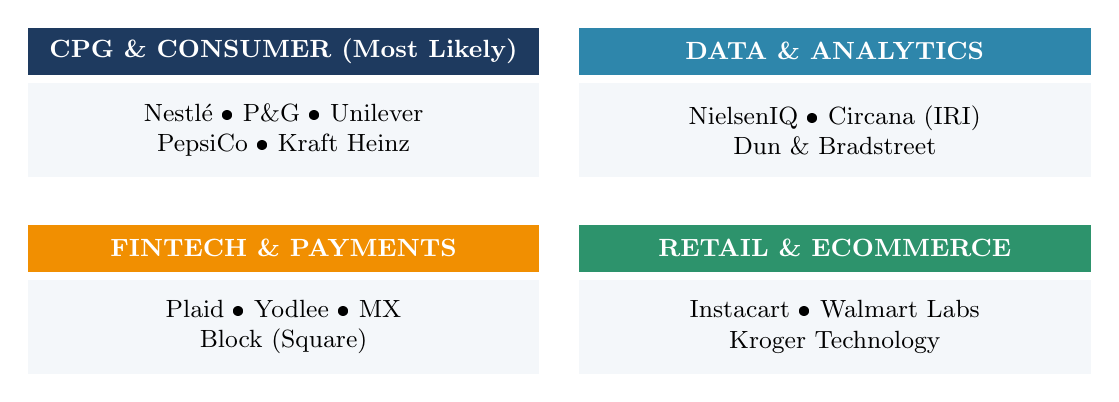
\begin{tikzpicture}
    % CPG
    \node[fill=miloprimary, text=white, font=\small\bfseries, minimum width=6.5cm, minimum height=0.6cm] at (-3.5, 1.5) {CPG \& CONSUMER (Most Likely)};
    \node[fill=milolight, font=\small, minimum width=6.5cm, minimum height=1.2cm, align=center] at (-3.5, 0.5) {Nestl\'{e} \textbullet\ P\&G \textbullet\ Unilever\\PepsiCo \textbullet\ Kraft Heinz};

    % Data
    \node[fill=milosecondary, text=white, font=\small\bfseries, minimum width=6.5cm, minimum height=0.6cm] at (3.5, 1.5) {DATA \& ANALYTICS};
    \node[fill=milolight, font=\small, minimum width=6.5cm, minimum height=1.2cm, align=center] at (3.5, 0.5) {NielsenIQ \textbullet\ Circana (IRI)\\Dun \& Bradstreet};

    % Fintech
    \node[fill=miloaccent, text=white, font=\small\bfseries, minimum width=6.5cm, minimum height=0.6cm] at (-3.5, -1) {FINTECH \& PAYMENTS};
    \node[fill=milolight, font=\small, minimum width=6.5cm, minimum height=1.2cm, align=center] at (-3.5, -2) {Plaid \textbullet\ Yodlee \textbullet\ MX\\Block (Square)};

    % Retail
    \node[fill=milogreen, text=white, font=\small\bfseries, minimum width=6.5cm, minimum height=0.6cm] at (3.5, -1) {RETAIL \& ECOMMERCE};
    \node[fill=milolight, font=\small, minimum width=6.5cm, minimum height=1.2cm, align=center] at (3.5, -2) {Instacart \textbullet\ Walmart Labs\\Kroger Technology};
\end{tikzpicture}
\end{center}

\subsubsection{Exit Valuation Range (Conservative)}

\begin{center}
\begin{tabular}{L{3cm} C{2.5cm} R{3cm} C{2.5cm}}
    \toprule
    \rowcolor{miloprimary}
    \textcolor{white}{\textbf{Scenario}} & \textcolor{white}{\textbf{Multiple}} & \textcolor{white}{\textbf{Valuation}} & \textcolor{white}{\textbf{Seed Return}}\\
    \midrule
    Conservative & 5x & \$12M & 3-4x\\
    \rowcolor{miloaccent!20}
    \textbf{Base Case} & \textbf{6x} & \textbf{\$14.4M} & \textbf{6-8x}\\
    Moderate & 8x & \$19.2M & 10-12x\\
    \rowcolor{milolight}
    Optimistic & 10x & \$24M & 12-15x\\
    \bottomrule
\end{tabular}
\end{center}

\newpage

% ============================================================================
% SECTION 12: STRATEGIC ROADMAP
% ============================================================================
\section{Strategic Roadmap}

\subsection{Milestone Timeline}

\begin{center}
\begin{tikzpicture}[
    milestone/.style={draw=milosecondary, fill=milolight, rounded corners=8pt, minimum width=3.8cm, minimum height=5cm, align=center, font=\small}
]
    % Timeline header
    \node[font=\large\bfseries, color=miloprimary] at (0, 4.5) {STRATEGIC MILESTONES};

    % Phase boxes
    \node[milestone] (p1) at (-6, 0) {
        \textbf{\textcolor{miloprimary}{2026 Q2-Q3}}\\
        {\footnotesize FOUNDATION}\\[8pt]
        \faIcon{check} Close Seed Round\\
        \faIcon{check} GDPR Compliance\\
        \faIcon{check} App Store Launch\\
        \faIcon{check} 1K-1.5K MAU\\
        \faIcon{check} Beta Validation
    };

    \node[milestone] (p2) at (-2, 0) {
        \textbf{\textcolor{miloprimary}{2026 Q4 - 2027 Q2}}\\
        {\footnotesize VALIDATION}\\[8pt]
        \faIcon{check} Achieve 5K MAU\\
        \faIcon{check} First B2B Revenue\\
        \faIcon{check} \$30K MRR\\
        \faIcon{check} 2+ Enterprise Pilots\\
        \faIcon{check} Prove Unit Economics
    };

    \node[milestone] (p3) at (2, 0) {
        \textbf{\textcolor{miloprimary}{2027 Q3 - 2028}}\\
        {\footnotesize SCALE}\\[8pt]
        \faIcon{check} Android Launch\\
        \faIcon{check} UK Expansion\\
        \faIcon{check} 15K MAU\\
        \faIcon{check} Series A Prep\\
        \faIcon{check} Team Growth
    };

    \node[milestone] (p4) at (6, 0) {
        \textbf{\textcolor{miloprimary}{2028-2029}}\\
        {\footnotesize EXIT OPTIONALITY}\\[8pt]
        \faIcon{check} 25K MAU\\
        \faIcon{check} \$2.4M ARR\\
        \faIcon{check} 58\% Op. Margin\\
        \faIcon{check} Strategic Acquisition\\
        {\footnotesize or Series A}
    };

    % Connecting arrows
    \draw[-{Stealth[length=4mm]}, thick, miloaccent] (p1) -- (p2);
    \draw[-{Stealth[length=4mm]}, thick, miloaccent] (p2) -- (p3);
    \draw[-{Stealth[length=4mm]}, thick, miloaccent] (p3) -- (p4);
\end{tikzpicture}
\end{center}

\subsection{Key Milestones}

\begin{center}
\begin{tabular}{L{2.5cm} L{5cm} L{5.5cm}}
    \toprule
    \rowcolor{miloprimary}
    \textcolor{white}{\textbf{Period}} & \textcolor{white}{\textbf{Primary Goals}} & \textcolor{white}{\textbf{Success Metrics}}\\
    \midrule
    \textbf{M1-6} & Foundation \& Launch & 1.5K MAU, GDPR compliance, app live\\
    \rowcolor{milolight}
    \textbf{M7-12} & Growth \& Validation & 3.5K MAU, 2 B2B pilots, \$15K MRR\\
    \textbf{M13-24} & Scale \& Profitability & 9K MAU, \$50K MRR, cash flow positive\\
    \rowcolor{milolight}
    \textbf{M25-36} & Expansion & 25K MAU, \$200K MRR, exit-ready\\
    \bottomrule
\end{tabular}
\end{center}

\subsection{Critical Success Factors}

\begin{accentbox}
\begin{center}
{\Large\bfseries\textcolor{miloaccent}{CRITICAL SUCCESS FACTORS}}
\end{center}

\vspace{10pt}

\begin{enumerate}[leftmargin=20pt, itemsep=8pt]
    \item \textbf{GDPR COMPLIANCE} (Non-Negotiable)\\
    {\small Must achieve before launch --- blocks 52\% of revenue otherwise}

    \item \textbf{TRIAL CONVERSION}\\
    {\small Achieving 15\%+ trial-to-paid --- drives all B2C revenue}

    \item \textbf{DATA CONSENT}\\
    {\small Achieving 40\%+ opt-in --- enables B2B revenue stream}

    \item \textbf{UNIT ECONOMICS}\\
    {\small Maintaining CAC <\$20 and LTV:CAC >3:1 --- validates scalability}

    \item \textbf{B2B CAPABILITY}\\
    {\small Building sales function --- 52\% of revenue depends on this}
\end{enumerate}
\end{accentbox}

\newpage

% ============================================================================
% SECTION 13: APPENDIX
% ============================================================================
\section{Appendix}

\subsection{Financial Model Summary}

\begin{center}
\begin{tabular}{L{4cm} R{2cm} R{2cm} R{2cm} R{2.5cm}}
    \toprule
    \rowcolor{miloprimary}
    \textcolor{white}{\textbf{Line Item}} & \textcolor{white}{\textbf{Y1}} & \textcolor{white}{\textbf{Y2}} & \textcolor{white}{\textbf{Y3}} & \textcolor{white}{\textbf{3-Year Total}}\\
    \midrule
    \textbf{Revenue} & \$228K & \$1.1M & \$2.4M & \$3.73M\\
    \rowcolor{milolight}
    COGS/Variable & (\$40K) & (\$130K) & (\$255K) & (\$425K)\\
    \textbf{Gross Profit} & \$188K & \$970K & \$2.15M & \$3.3M\\
    \rowcolor{milolight}
    Gross Margin & 82.5\% & 88.2\% & 89.4\% & 88.6\%\\
    Operating Expenses & (\$260K) & (\$552K) & (\$755K) & (\$1.57M)\\
    \rowcolor{milogreen!20}
    \textbf{Operating Profit} & (\$72K) & \$418K & \$1.39M & \$1.74M\\
    \rowcolor{milolight}
    Operating Margin & -31.6\% & 38.0\% & 58.0\% & 46.6\%\\
    \bottomrule
\end{tabular}
\end{center}

\subsection{Key Assumptions (Conservative)}

\begin{center}
\begin{tabular}{L{4cm} L{3cm} L{5.5cm}}
    \toprule
    \rowcolor{miloprimary}
    \textcolor{white}{\textbf{Assumption}} & \textcolor{white}{\textbf{Value}} & \textcolor{white}{\textbf{Rationale}}\\
    \midrule
    Year 3 Paid Users & 9,720 & 15\% trial conversion, 80/20 tier mix\\
    \rowcolor{milolight}
    Trial Conversion & 15\% & Below industry average (20-25\%)\\
    Data Consent Rate & 40\% & Below industry average (50-60\%)\\
    \rowcolor{milolight}
    Monthly Churn & 10\% & Above industry average (5-8\%)\\
    B2B Deal Size & \$75K avg & Mid-market focus, conservative\\
    \rowcolor{milolight}
    Veryfi Cost & \$0.08/receipt & Current contracted rate\\
    \bottomrule
\end{tabular}
\end{center}

\subsection{Document References}

This executive summary synthesizes analysis from:

\begin{itemize}[leftmargin=20pt, itemsep=3pt]
    \item Pricing Strategy v2.0 (14-day trial, Gold/Platinum tiers)
    \item Financial Projections (Conservative model)
    \item Risk Assessment \& Mitigation Strategies
    \item Competitive Analysis \& SWOT
    \item GDPR Compliance Assessment
    \item Marketing Strategy (Conservative budget)
    \item Data Monetization Strategy
    \item Cost Analysis \& Unit Economics
\end{itemize}

\newpage

% ============================================================================
% CONCLUSION
% ============================================================================
\section*{Conclusion}
\addcontentsline{toc}{section}{Conclusion}

\begin{keymetricbox}
\begin{center}
{\Large\bfseries INVESTMENT RECOMMENDATION}\\[20pt]


\begin{tikzpicture}
    \node[fill=miloaccent, text=white, font=\Huge\bfseries, minimum width=5cm, minimum height=2cm, rounded corners=10pt] {CAUTIOUS BUY};
\end{tikzpicture}

\vspace{15pt}

{\large MILO represents a category-creating opportunity with meaningful upside potential, tempered by execution risks that warrant conservative expectations.}
\end{center}
\end{keymetricbox}

\vspace{15pt}

\begin{minipage}[t]{0.48\textwidth}
\begin{successbox}
\textbf{\textcolor{milogreen}{STRENGTHS:}}
\begin{itemize}[leftmargin=15pt, itemsep=3pt]
    \item[\textcolor{milogreen}{\faIcon{check}}] Unique value proposition in growing markets
    \item[\textcolor{milogreen}{\faIcon{check}}] Viable unit economics (3:1+ LTV:CAC)
    \item[\textcolor{milogreen}{\faIcon{check}}] Diversified revenue reduces single-point-of-failure risk
    \item[\textcolor{milogreen}{\faIcon{check}}] Privacy-first architecture enables premium B2B positioning
\end{itemize}
\end{successbox}
\end{minipage}
\hfill
\begin{minipage}[t]{0.48\textwidth}
\begin{riskbox}
\textbf{\textcolor{milored}{RISKS:}}
\begin{itemize}[leftmargin=15pt, itemsep=3pt]
    \item[\textcolor{milored}{\faIcon{times}}] GDPR compliance required before launch
    \item[\textcolor{milored}{\faIcon{times}}] B2B revenue (52\%) depends on consent rates
    \item[\textcolor{milored}{\faIcon{times}}] No existing user base requires acquisition spending
    \item[\textcolor{milored}{\faIcon{times}}] Subscription fatigue trend may impact conversion
\end{itemize}
\end{riskbox}
\end{minipage}

\vspace{20pt}

\begin{accentbox}
\begin{center}
The \textbf{\$400K-\$600K seed investment} offers \textbf{6-10x return potential} under conservative assumptions, with meaningful downside protection through early profitability focus and diversified revenue streams.

\vspace{10pt}
{\Large\bfseries\textcolor{miloaccent}{RECOMMENDATION: Invest with clear milestones and capital tranches}}
\end{center}
\end{accentbox}

\vspace{30pt}

\begin{center}
\rule{0.6\textwidth}{0.5pt}\\[20pt]
{\Large\textbf{\textcolor{miloprimary}{DeepmAInd B.V.}}}\\[10pt]
{\itshape Building the future of wellness-aware spending intelligence}\\[30pt]

{\footnotesize\color{milogray}
This document is confidential and intended for authorized recipients only.\\
Forward-looking statements are based on current expectations and assumptions.\\
Actual results may vary materially. All projections use conservative assumptions.\\[15pt]
\textbf{Document Version:} 2.0 (Conservative Model) | \textbf{Last Updated:} January 28, 2026 | \textbf{Prepared for:} CEO Review
}
\end{center}

\end{document}
